% Chapter 2

\chapter{Introduction to PFAS}

\label{Chapter2}

%---------------------------------------------------------------------------------------- 
\newcommand{\keyword}[1]{\textbf{#1}}
\newcommand{\tabhead}[1]{\textbf{#1}}
\newcommand{\code}[1]{\texttt{#1}}
\newcommand{\file}[1]{\texttt{\bfseries#1}}
\newcommand{\option}[1]{\texttt{\itshape#1}}

%----------------------------------------------------------------------------------------

\section{Definition and Structure}

PFAS (Per- and Polyfluoroalkyl Substances) are organic compounds characterized by a carbon chain bonded to fluorine atoms. According to the latest definition by the Organization for Economic Co-operation and Development (OECD), PFAS are fluorinated substances containing at least one fully fluorinated methyl or methylene carbon atom \cite{2}. PFAS can be categorized into short-chain (≤ 7 carbon atoms) and long-chain (≥ 8 carbon atoms) compounds, with the latter often referred to as legacy compounds due to their long history of study. Among the most extensively researched long-chain PFAS are perfluorooctane sulfonate (PFOS) and perfluorooctanoic acid (PFOA) with their production discontinued in some countries, for example in the United States during the 2000s, because of their harmful health effects\cite{2} \cite{3}.

The chemical structure of PFAS, particularly the carbon-fluorine (C-F) bonds, is among the strongest in organic chemistry. This bond strength contributes to the high resistance of PFAS to degradation, enabling them to persist in both the environment and the human body, where they are challenging to eliminate. PFAS are non-flammable, non-corrosive, and do not burn, degrade, or react easily with other chemicals. Typically, PFAS molecules possess both hydrophobic and hydrophilic ends, contributing to their unique surfactant properties. The long half-lives of these compounds mean they accumulate over time, further complicating efforts to manage their impact on health and the environment. Although the production of certain PFAS, such as PFOA and PFOS, was discontinued in some countries like the United States during the 2000s due to their harmful health effects, these compounds continue to pose significant risks \cite{PFOA_PFOS_risk}.


\begin{figure}[H]
\centering
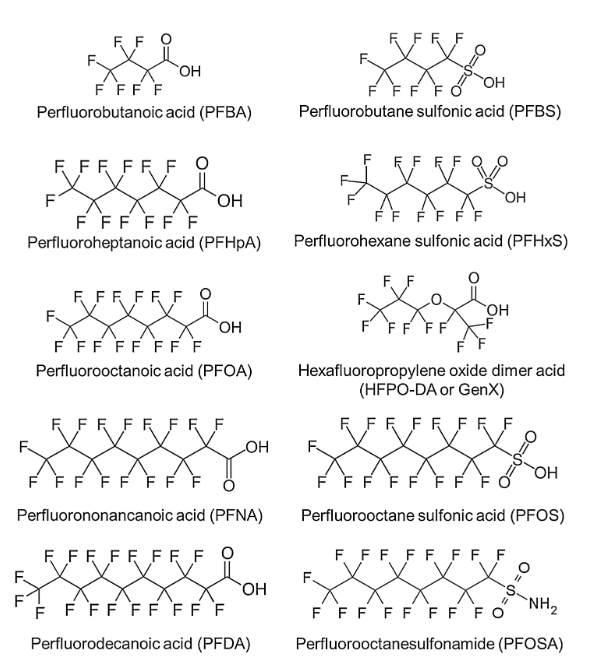
\includegraphics[width=\textwidth,height=\textheight,keepaspectratio]{Figures/structure_chapter_2.png}
\caption{2D Chemical structures of sample PFAS and similar compounds.}
\label{structure_chapter_2}
\FloatBarrier
\end{figure}


%----------------------------------------------------------------------------------------

\section{Uses and Potential Risks}

PFAS are a group of synthetic compounds widely used in industrial processes due to their resistance to degradation, surfactant properties, and thermal and flame resistance. Their water- and grease-resistant properties make them common in food packaging, non-stick cookware, and waterproof textiles. Beyond these applications, PFAS are also found in products such as paints, adhesives, electrical wire insulation, detergents, fire-resistant materials, carpets, and even cosmetics \cite{3} \cite{4}.

One of the most concerning effects of PFAS exposure is their potential impact on thyroid health. Thyroid hormones are crucial for regulating metabolism, and thyroid function is closely linked to cardiovascular health, fertility, and fetal neurodevelopment. Studies have suggested that PFAS may disrupt thyroid hormone systems, potentially affecting pregnancy outcomes and fetal-child development \cite{3}.

%----------------------------------------------------------------------------------------

\section{Environmental and Health Concerns}

The widespread use of PFAS across various industries, coupled with their chemical stability, has led to significant environmental contamination. PFAS have been detected in surface water, groundwater, soil, and air. Their solubility in water and resistance to degradation allow them to travel long distances from their original source, leading to widespread distribution in the environment. [\href{https://www.diva-portal.org/smash/get/diva2:892150/FULLTEXT01.pdf}{Long-range transport of
per- and polyfluorinated
substances to Sweden}]

Recent epidemiological studies have linked exposure to certain PFAS compounds with various adverse health outcomes. These health risks are compounded by the fact that PFAS can accumulate in the human body over time, particularly in blood, liver, and kidneys, due to their long biological half-lives. Consequently, even low-level exposure to PFAS over an extended period can result in significant health impacts thanks to the persistent nature. Many legacy PFAS, such as PFOA and PFOS, have accumulated in the environment, animals, and humans. Mixtures of both legacy and newer PFAS continue to be found throughout the environment, including in food and water supplies worldwide. The biological half-lives of legacy PFAS in human serum are approximately 4 years for PFOA, 5 years for PFOS, and 8.5 years for PFHxS. For newer PFAS, the half-life is not well understood; however, studies suggest that the excretion rates are significantly faster \cite{4}.


To completely eliminate fluoride contamination, complete defluoridation or mineralization of PFAS is necessary. However, currently available technologies can only partially defluorinate a limited range of PFAS. In 2023, the U.S. Environmental Protection Agency set new drinking water standards for perfluorooctanesulfonic acid (PFOS) and perfluorooctanoic acid (PFOA) at 4.0 ppt. To achieve this almost zero standard, technological innovations that enable complete defluorination (DeF), rather than just degradation, of parent PFAS compounds are needed. DeF specifically refers to the percentage of fluoride ions released from PFAS molecules. Achieving complete DeF is crucial, as partial DeF can result in the formation of potentially more harmful and persistent shorter chain products by that are more likely to bioaccumulate in animals and human \cite{6}.

%----------------------------------------------------------------------------------------


\section{Regulatory Challenges and Research Directions}

Given the persistence and toxicity of PFAS, regulatory agencies worldwide have begun to implement guidelines and regulations to limit PFAS exposure. For example, the United States Environmental Protection Agency (EPA) has established health advisories for PFOA and PFOS in drinking water, although these advisories are non-enforceable and are currently under review for potential revision. Similarly, several countries in the European Union have restricted the use of certain PFAS in consumer products and industrial applications. Despite these efforts, the sheer number of PFAS compounds, coupled with the lack of comprehensive toxicological data for many of them, presents significant challenges for regulators \cite{PFAS_regulators} \cite{PFAS_regulators_2} \cite{PFAS_regulators_3}.

Ongoing research is focused on developing more effective methods for detecting and quantifying PFAS in environmental samples and exploring potential remediation strategies. Analytical techniques such as liquid chromatography-mass spectrometry (LC-MS/MS) have become the gold standard for PFAS detection due to their sensitivity and specificity \cite{PFAS_detection_1}, \cite{PFAS_detection_2}, \cite{PFAS_detection_3}, \cite{PFAS_detection_4}. However, detecting PFAS at environmentally relevant concentrations remains a challenge, particularly for emerging PFAS compounds that are not well-characterized.

In terms of remediation, traditional water treatment technologies, such as activated carbon filtration and ion exchange, have shown some efficacy in removing PFAS from contaminated water sources. However, these methods are often limited in their ability to address the full spectrum of PFAS compounds present in the environment. Advanced treatment methods, including high-pressure membrane filtration, advanced oxidation processes, and electrochemical degradation, are being investigated as potential solutions to this problem \cite{PFAS_membrane_filtration}, \cite{PFAS_oxidation_1}, \cite{PFAS_oxidation_2}.

%----------------------------------------------------------------------------------------